\chapter{Data Analysis and Preprocessing}\label{chap:data}

As we mentioned in Chapter \ref{chap:introduction}, our work is based on a
dataset collected for a study on the effects of visualizing the progress of
weight loss using a \gls{vr} headset during a weight loss treatment .

\section{3D body model dataset under dietetic treatment}

Our dataset comprises approximately 400 sessions obtained from 80 distinct
patients. These sessions, recorded at irregular intervals, incorporate a 3D
scan of the patient and a multitude of other measurements such as weight,
height, body fat percentage, and more.

\begin{table}[h]
	\centering
	\begin{tabular}{ l l l }
		\toprule
		Type                               & Source                                                                                         & Measurement (unit)                        \\
		\midrule
		\multirow{3}{*}{Anthropometric}    & \multirow{3}{4cm}{Flexible measuring tape}                                                     & Wrist (cm)                                \\
		                                   &                                                                                                & Waist (cm)                                \\
		                                   &                                                                                                & Hip (cm)                                  \\
		\midrule

		\multirow{6}{*}{Body composition}  & \multirow{6}{4cm}{Tanita\textregistered\ MC 780-P MA and Seca\textregistered\ 213 stadiometer} & Fat per limb and trunk (\%)               \\
		                                   &                                                                                                & Muscle per limb and trunk (\%)            \\
		                                   &                                                                                                & Total fat and muscle (\%)                 \\
		                                   &                                                                                                & Visceral fat area (cm\textsuperscript{2}) \\
		                                   &                                                                                                & Weight (kg)                               \\
		                                   &                                                                                                & Height (m)                                \\
		\midrule

		\multirow{3}{*}{Other, Lifestyle}  & \multirow{3}{4cm}{Interview}                                                                   & Activity   (score)                        \\
		                                   &                                                                                                & Gender                                    \\
		                                   &                                                                                                & Age (years)                               \\

		\midrule

		\multirow{3}{*}{Blood (capillary)} & \multirow{3}{4cm}{Accutrend\textregistered\ Plus}                                              & Glucose (mg/dL)                           \\
		                                   &                                                                                                & Cholesterol (mg/dL)                       \\
		                                   &                                                                                                & Triglycerides (mg/dL)                     \\

		\midrule

		\multirow{2}{*}{Blood pressure}    & \multirow{2}{4cm}{Omron\textregistered\ M3}                                                    & Systolic pressure (mmHg)                  \\
		                                   &

		                                   & Diastolic pressure (mmHg)                                                                                                                  \\
		\bottomrule

	\end{tabular}
	\caption{Measurements collected from each session \citep{10045_124160}.}
\end{table}

The raw data, however, required extensive cleaning before it could be analyzed.
We encountered sessions missing certain measurements and numerous data
outliers. After our data cleaning process, we were left with approximately 200
viable sessions.

\begin{figure}[h]
	\centering
	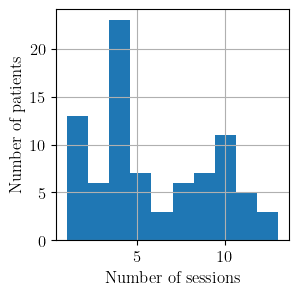
\includegraphics{files/sessions_per_patient}
	\caption{Variation in the number of sessions per patient.}
	\label{fig:sessions-per-patient}
\end{figure}

As Figure~\ref{fig:sessions-per-patient} illustrates, the number of sessions
per patient varied significantly, with some patients attending only a single
session and others attending over ten. Given that neural networks necessitate
uniform input shapes, we were faced with a challenge. We'll elaborate on how we
tackled this problem in Chapter \ref{chap:nn}.

\section{Data Cleaning and Outlier Detection}

A data cleaning pipeline was constructed utilizing the \gls{pandas} library.
Essential steps encompassed missing data treatment, duplicate removal, and
variable unit standardization.

We indexed our dataset with a multi-index that included the patient's id and
the session number. This system facilitated patient-specific data iteration and
simplified the process of pinpointing patient data discrepancies.

Upon scrutinizing plotted data, we discovered that the decimal separator was a
common source of errors. Many measurements appeared to be inflated by a factor
of 10, prompting us to devise tailored rules to correct this. Additional rules
were implemented to identify and discard out-of-range values or those
conflicting with other measurements. These rules included:

\begin{itemize}
	\item Small variation between measurements of different limbs, such as muscle or fat
	      percentage discrepancies between left and right arms.
	\item Ensuring that the combined muscle and fat percentages do not exceed 100\%.
	\item Verifying that the fat and muscle percentage levels individually stay below
	      100\% --- values exceeding this typically indicate a measurement inflated by a
	      factor of 10.
\end{itemize}

Despite these rectifications, some outliers persisted. We experimented with a
system that flagged dramatic session-to-session changes, but found it too
susceptible to false positives. Eventually, we opted to manually inspect the
data, flagging conspicuous outliers for removal.

\begin{figure}[h]
	\centering
	\begin{subfigure}{\textwidth}
		\centering
		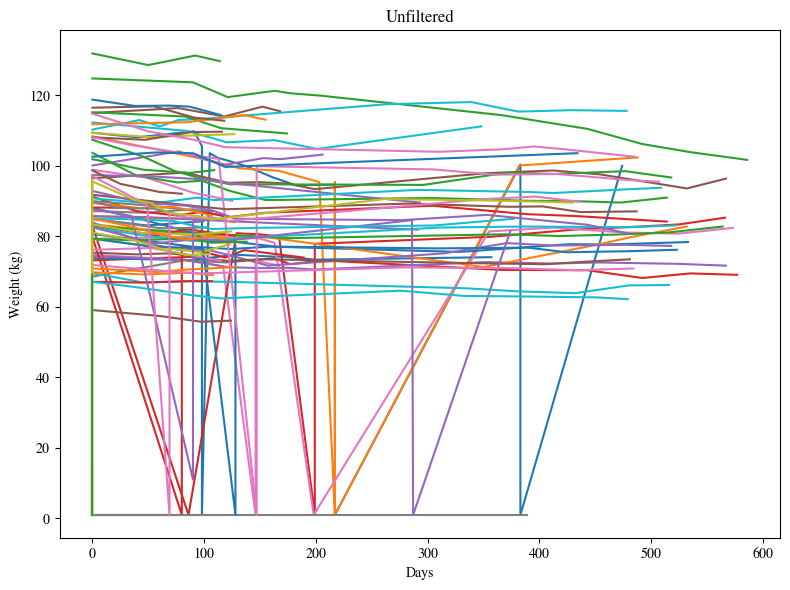
\includegraphics[width=0.8\textwidth]{files/weight_unfiltered}
		\caption{Raw weight.}
	\end{subfigure}
	\begin{subfigure}{\textwidth}
		\centering
		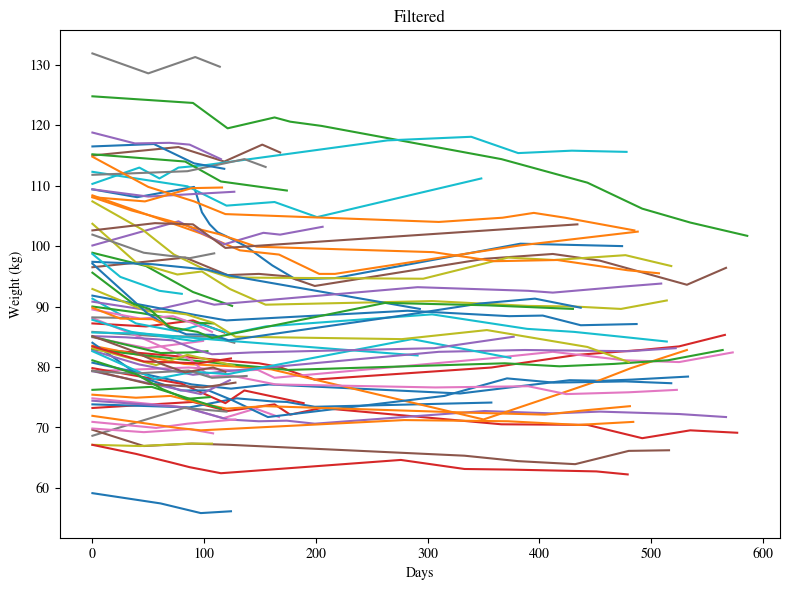
\includegraphics[width=0.8\textwidth]{files/weight_filtered}
		\caption{Filtered weight.}
	\end{subfigure}
	\caption{Weight measurements pre and post filtering.}
\end{figure}

\section{SMPL for Body Representation}

In our study, we found it crucial to accurately represent the human body's
complex and varied structure. This necessity led us to adopt the \gls{smpl}
model. \gls{smpl} is a versatile and practical mathematical model for capturing
a wide range of human body shapes and poses. It provides a parametric approach
to represent the body shape and pose in a low-dimensional linear space, thus
making it a valuable asset in our research.

\gls{smpl} characterizes the human body using two sets of parameters: shape ($\beta$)
and pose ($\theta$). The shape parameters ($\beta$) are derived from a
principal component analysis of the shapes in a training set. \gls{smpl} uses a
vector of 10 shape coefficients that define the primary modes of shape
variation. These coefficients cover a wide array of human body shapes, allowing
us to capture a comprehensive view of a patient's body structure.

\begin{figure}[H]
	\centering
	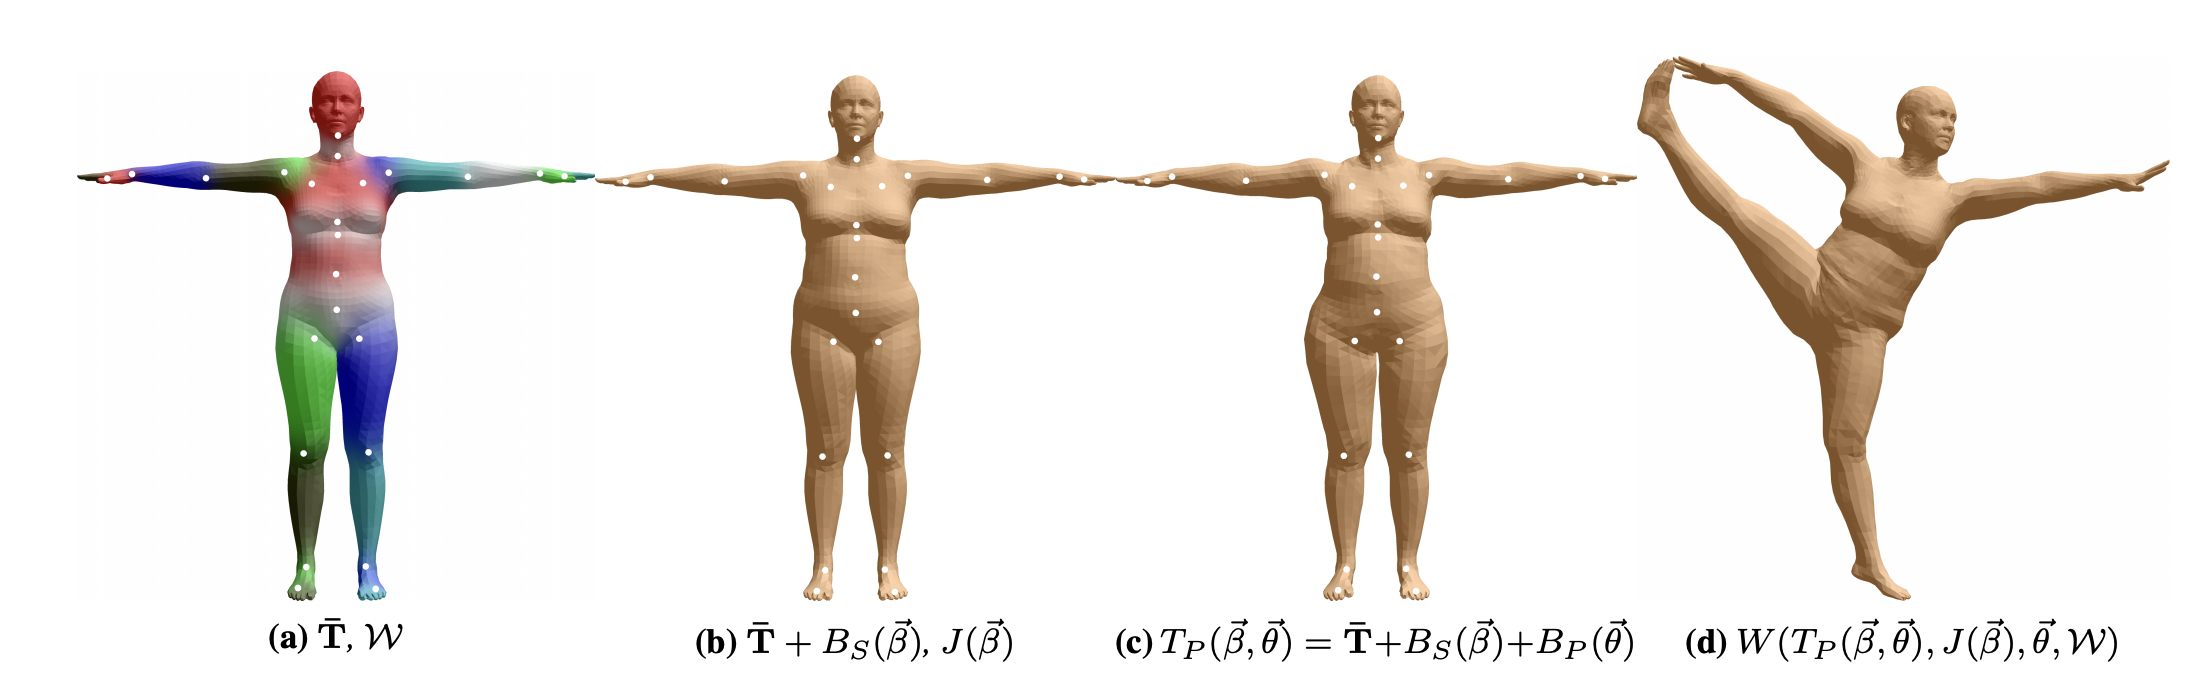
\includegraphics[width=\textwidth]{files/SMPL_formulation}
	\caption{SMPL model \citep{meshcapade}}
	\label{fig:SMPL_formulation}
\end{figure}

On the other hand, the pose parameters ($\theta$) represent the orientation of
the body's joints. This parameter encodes the body's pose into 72 pose
coefficients. While the pose parameters offer a detailed portrayal of body
position, our interest primarily lies in the body shape. Therefore, we focus on
the shape parameters for our study.

\gls{smpl} serves as an ideal fit for our problem due to its compact, continuous, and
differentiable nature. The model's low-dimensionality reduces computational
complexity, making it a practical choice for large-scale analysis. Moreover,
the differentiable nature of the model facilitates gradient-based optimization
methods, essential for precise parameter estimation. The model's continuous
representation also allows for a seamless transition between different body
shapes, further enhancing the realism and accuracy of the body representations.

We extracted \gls{smpl} parameters — shape ($\beta$) and pose ($\theta$) — from
the 3D scans using a custom minimization algorithm \citep{estimation:2023}.
This method encompassed the following stages:

\begin{figure}[H]
	\centering
	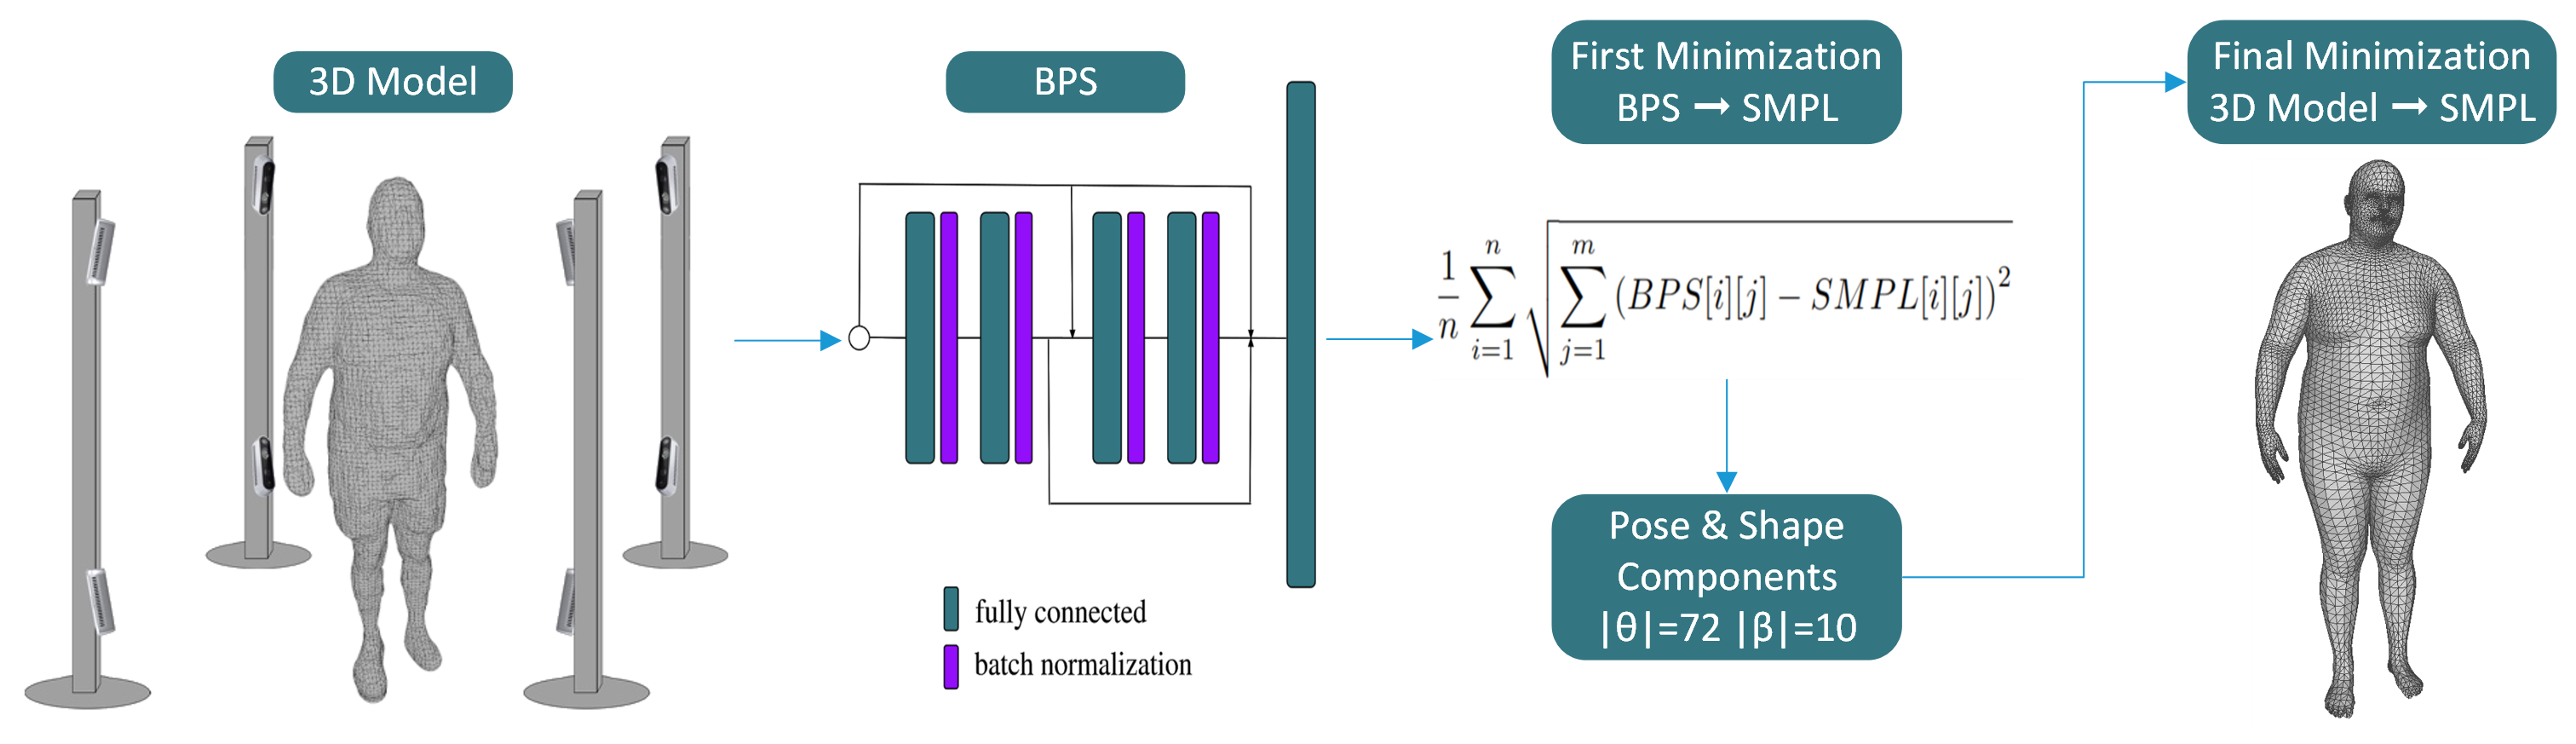
\includegraphics[width=\textwidth]{files/pipeline_smpl.png}
	\caption{Our pipeline for extracting SMPL parameters from 3D scans.}
\end{figure}

\begin{itemize}
	\item Acquiring and Preprocessing of 3D Data: The Tech4Diet project's system, fitted
	      with 13 Intel RealSense RGB-D cameras, was used to capture the 3D data (Figure
	      \ref{fig:cameras_scan}). This data was then preprocessed to minimize noise and
	      optimize 3D scan alignment.

	\item Estimating an Intermediate Template using a BPS Neural Network: The \gls{bps}
	      method was used to generate an intermediate 3D model by encoding a set of
	      points into fixed-distance representations. A DenseNet neural network then took
	      this \gls{bps} representation as input to predict the vertex positions of a
	      template resembling the input point cloud.

	\item First Minimization: \gls{bps} to \gls{smpl}: We minimized the pose and shape
	      parameters of the \gls{smpl} model to align it with the template created by the
	      \gls{bps}.

	\item Second Minimization: 3D Scan to \gls{smpl}: A second minimization was performed
	      to align the \gls{smpl} model with the 3D scan from the RGB-D sensors. We
	      proposed an algorithm to enhance the speed and accuracy of this process by
	      segmenting the model into body parts, applying rigid registration, and then
	      using a custom minimization function that considered both distance and normal
	      angles.
\end{itemize}

\begin{figure}[H]
	\centering
	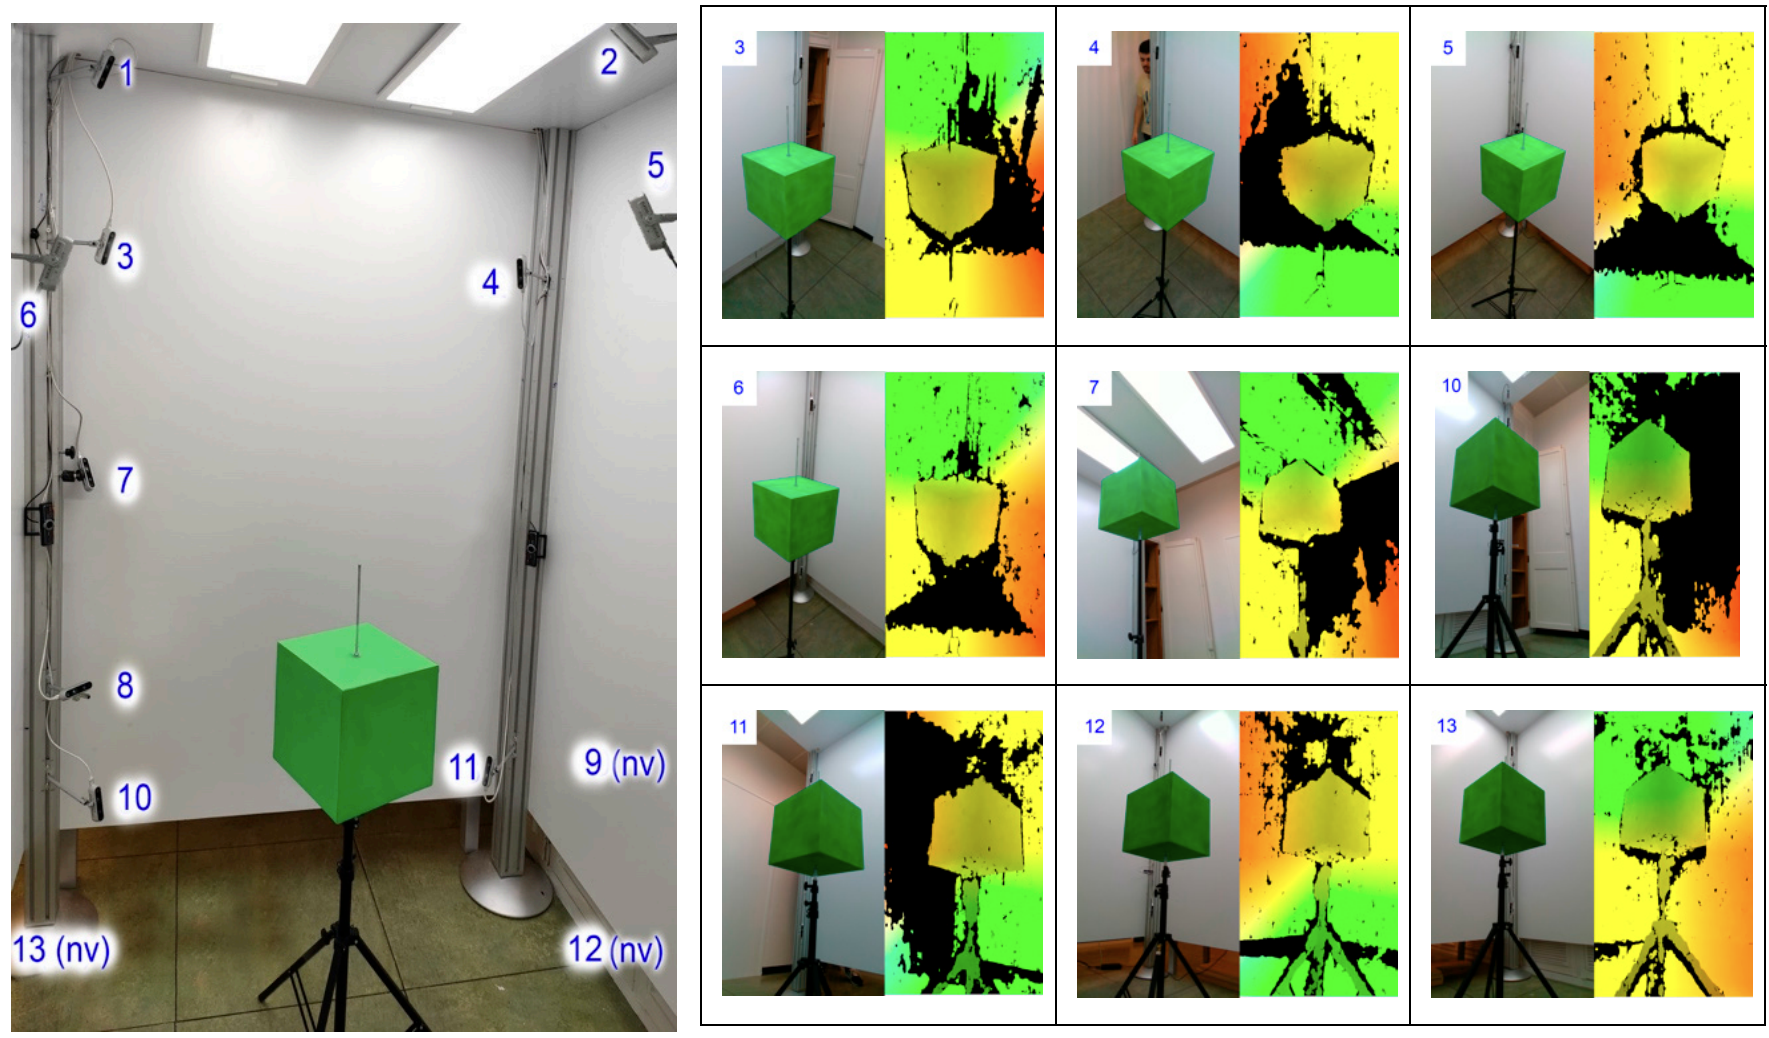
\includegraphics[width=\textwidth]{files/cameras_scan.png}
	\caption{Our 3D scanning system.}
	\label{fig:cameras_scan}
\end{figure}

Figures \ref{fig:beta-1-vis} to \ref{fig:beta-10-vis} (in the Annex
\ref{chap:annex1}) demonstrate the effects of shape parameter variations.
Although we employed a scale of 3 to amplify their effects for visualization,
actual values are significantly lower. $\beta_1$ regulates the overall body
height, while $\beta_2$ is highly correlated with the body mass index.

\begin{table}[h]
	\centering
	\begin{tabular}{c | c c c c c c c c c c}
		\toprule
		     & $\beta_1$ & $\beta_2$ & $\beta_3$ & $\beta_4$ & $\beta_5$ & $\beta_6$ & $\beta_7$ & $\beta_8$ & $\beta_9$ & $\beta_{10}$ \\
		\midrule
		mean & 0.88      & -0.73     & 0.34      & 0.01      & 0.06      & 0.06      & 0.11      & 0.02      & 0.01      & 0.11         \\

		std  & 0.97      & 0.78      & 0.26      & 0.21      & 0.12      & 0.13      & 0.08      & 0.03      & 0.03      & 0.08         \\

		min  & -1.42     & -2.57     & -0.64     & -0.65     & -0.23     & -0.25     & -0.14     & -0.07     & -0.08     &
		-0.17                                                                                                                           \\

		25\% & 0.12      & -1.26     & 0.15      & -0.14     & -0.01     & -0.02     & 0.04      & 0.00      & -0.01     & 0.06         \\

		50\% & 0.94      & -0.69     & 0.36      & 0.03      & 0.04      & 0.02      & 0.11      & 0.02      & 0.01      & 0.11         \\

		75\% & 1.66      & -0.20     & 0.52      & 0.17      & 0.14      & 0.14      & 0.16      & 0.04      & 0.04      & 0.17         \\

		max  & 2.90      & 2.96      & 0.97      & 0.45      & 0.39      & 0.47      & 0.36      & 0.13      & 0.16      & 0.30         \\
		\bottomrule
	\end{tabular}
	\caption{Statistics of the shape parameters.}
\end{table}

\section{Exploring Additional Datasets}

Finding the right data is like searching for a needle in a haystack. It's a key
task if we want to improve our model, but it's also quite a challenge - and for
us, it was even more so due to a few reasons.

First, a lot of medical data isn't exactly out there for anyone to pick up and
use. Understandably, these datasets are kept private due to concerns around
confidentiality and privacy, which are of utmost importance when it comes to
health-related data. This makes these datasets not only hard to come by, but
also tough to gauge in terms of their usefulness for our work. It's hard to
tell if a dataset is going to be helpful if we can't even get a peek at what's
inside.

Second, there are open-source datasets with 3D scans of people. But there's a
catch: these datasets usually only provide a snapshot of a person's physique at
one point in time. They don't show how a person's body changes over time, which
is a key piece of the puzzle in our study on how diet interventions affect body
shape.

We also looked at datasets from fields like sports science or anthropometry.
These weren't specifically designed for studying body composition, but we
thought they might still have some useful data. However, the scope of the data,
the level of detail, and the lack of consistent body composition measurements
meant that these datasets didn't quite fit the bill either.

Considering these challenges, we decided to use our own data for training and
testing our model. To get around the limitations of our data, we used
techniques to artificially expand and diversify our dataset. We'll talk more
about how we did this in Chapter \ref{chap:nn}.